\begin{columns}[T]
  \begin{column}{0.55\textwidth}
    \textbf{The 5 FICO Score Factors:}
    \begin{enumerate}
      \item \textbf{Payment History (35\%)}: On-time bill payments.
      \item \textbf{Amounts Owed (30\%)}: Balances, including utilization.
      \item \textbf{Length of History (15\%)}: Age of credit accounts.
      \item \textbf{New Credit (10\%)}: Recent inquiries \& accounts.
      \item \textbf{Credit Mix (10\%)}: Variety of credit types.
    \end{enumerate}
  \end{column}
  \begin{column}{0.45\textwidth}
    \centering
    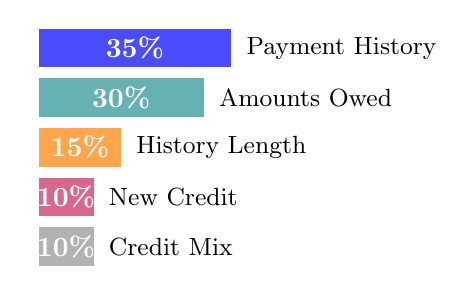
\begin{tikzpicture}[scale=0.70]
      % Horizontal stacked bar
      \fill[blue!70] (0,0) rectangle (3.5,0.7);
      \node at (1.75,0.35) {\color{white}\textbf{35\%}};

      \fill[teal!60] (0,-0.9) rectangle (3.0, -0.2);
      \node at (1.5,-0.55) {\color{white}\textbf{30\%}};

      \fill[orange!70] (0,-1.8) rectangle (1.5, -1.1);
      \node at (0.75,-1.45) {\color{white}\textbf{15\%}};

      \fill[purple!60] (0,-2.7) rectangle (1.0, -2.0);
      \node at (0.5,-2.35) {\color{white}\textbf{10\%}};

      \fill[gray!60] (0,-3.6) rectangle (1.0, -2.9);
      \node at (0.5,-3.25) {\color{white}\textbf{10\%}};

      \node[right] at (3.6,0.35) {\small Payment History};
      \node[right] at (3.1,-0.55) {\small Amounts Owed};
      \node[right] at (1.6,-1.45) {\small History Length};
      \node[right] at (1.1,-2.35) {\small New Credit};
      \node[right] at (1.1,-3.25) {\small Credit Mix};
    \end{tikzpicture}
  \end{column}
\end{columns}
